\documentclass[a4paper,11pt,oneside]{article}

\author{ J.R. Leeman} 
\title{Python Running Average Slope Package: rslope}

\usepackage{amsmath}
\usepackage{graphicx}
\usepackage{setspace}
\usepackage{indentfirst}
\usepackage{fullpage}
\usepackage{epstopdf}
\usepackage{listings}
\usepackage{color}
\usepackage{caption}

\definecolor{dkgreen}{rgb}{0,0.6,0}
\definecolor{gray}{rgb}{0.5,0.5,0.5}
\definecolor{mauve}{rgb}{0.58,0,0.82}

\lstset{frame=tb,
  language=Python,
  aboveskip=3mm,
  belowskip=3mm,
  showstringspaces=false,
  columns=flexible,
  basicstyle={\small\ttfamily},
  numbers=left,
  numberstyle=\tiny\color{gray},
  keywordstyle=\color{blue},
  commentstyle=\color{dkgreen},
  stringstyle=\color{mauve},
  breaklines=true,
  breakatwhitespace=true
  tabsize=3
}


\begin{document}
\maketitle
\newpage

\section{Purpose}
The rslope package was developed to take the running average slope (roughly a first derivative) of a given x,y set of datapoints.  A variable window size is used to allow use on data with various amounts of noise.  rslope can be used as a stand alone program to take input from a file or it may be imported into an existing Python program.

\section{Description}
rslope will compute the running average slope given two data vectors of equal length ($x$ and $y$) and a window size ($w$).  The window size is the number of data points on each side of the point under consideration to be used.  For example, a window setting of 5 would result in 11 points being considered: the data point we want the slope at and 5 datapoints on either side of it.  The full window is always $2w+1$.

rslope is based upon that a derivative is the slope of the local tangent line.  In fact if we set the window ($w$) to 1 and the program just considers only three data points (the point we are interested in, the one before, and the one after) we have a central difference type solution.  When dealing with data collected in a real system there is often too much noise and a simple solution provides no insight.  We use a window of data and fit a line to those points representing an approximate slope of the data.  Larger windows will result in data that is more smooth, but the slope averaged over more time, possibly erasing features that we desire to understand.  

Slope ($m$) of ($n$) datapoints is computed by equation \ref{slopes}.  For the entire dataset this is accomplished by keeping running totals of all the sums required and just adding and subtracting instead of recomputing the sum each step.  This saves significant time when large window sizes are used.  

\begin{equation}
m = \frac{\sum{xy} - \frac{\sum{x} \sum{y}}{n}}{\sum{x^2} - \frac{\left(\sum{x}\right)^2}{n}}
\label{slopes}
\end{equation}

For the first and last ($w$) datapoints the slope is computed over a smaller number ($n$) of points as the window is filling.  For example, a dataset with the window set to 2 will have 3 datapoints fit for the fist x,y pair, 4 datapoints fit for the second x,y pair, and finally a full window of 5 datapoints fit for the third x,y pair and all intermediate points.  As the end of the dataset is approached the reverse happens and the last x,y pair will be fit with 3 datapoints.

\section{Cautions}
A few cautions should be observed when using the rslope script:

\begin{enumerate}
\item The output will experience end effects for the first $w$ datapoints, where $w$ represents the window size.  After $w$ points the window size that the line is fit in is no longer changing and the result becomes stable.  
\item If the recording rate of data changes in the file the slopes will still be computed correctly (because we read the x and y channels in the fit), but likely the signal-to-noise ratio has changed.  This means the behavior of the output may change and should be carefully checked or the window size reconsidered.  The data could also be split into multiple files of uniform recording rate.
\end{enumerate}

\section{Usage}
rslope may be used in two modes: 1) as a stand alone program working on an input file, 2) as an imported  module in a python script.

In stand alone mode the code is called like a normal python argument with an argument for the file to be used.  The file should contain two columns of numbers, space delimited, with no headers.  Any headers or additional columns will cause the program to exit.\\\\ \emph{python rslope.py [filename]}

The rslope package can be imported to an existing script and the returned slope vector used.  Import with \emph{import rslope} or \emph{from rslope import rslope} and call with \emph{slopes = rslope.rslope(x,y,window=5)} or \emph{slopes = rslope(x,y,window=5)} respectively.  


\section{Verification}

Code verification was performed against Chris Marone's rslope program and two test functions with analytic derivatives.  The results of $f(x) = x^2$ (Fig.\ref{xsq_test}) and $f(x) = \text{sin}(x)$ (Fig.\ref{sin_test}) are included.  The expected results were obtained to numerical error with end effects that are known to exist for the first and last data points affected by a non-full window.

\noindent%
\begin{minipage}{\linewidth}
\makebox[\linewidth]{%
      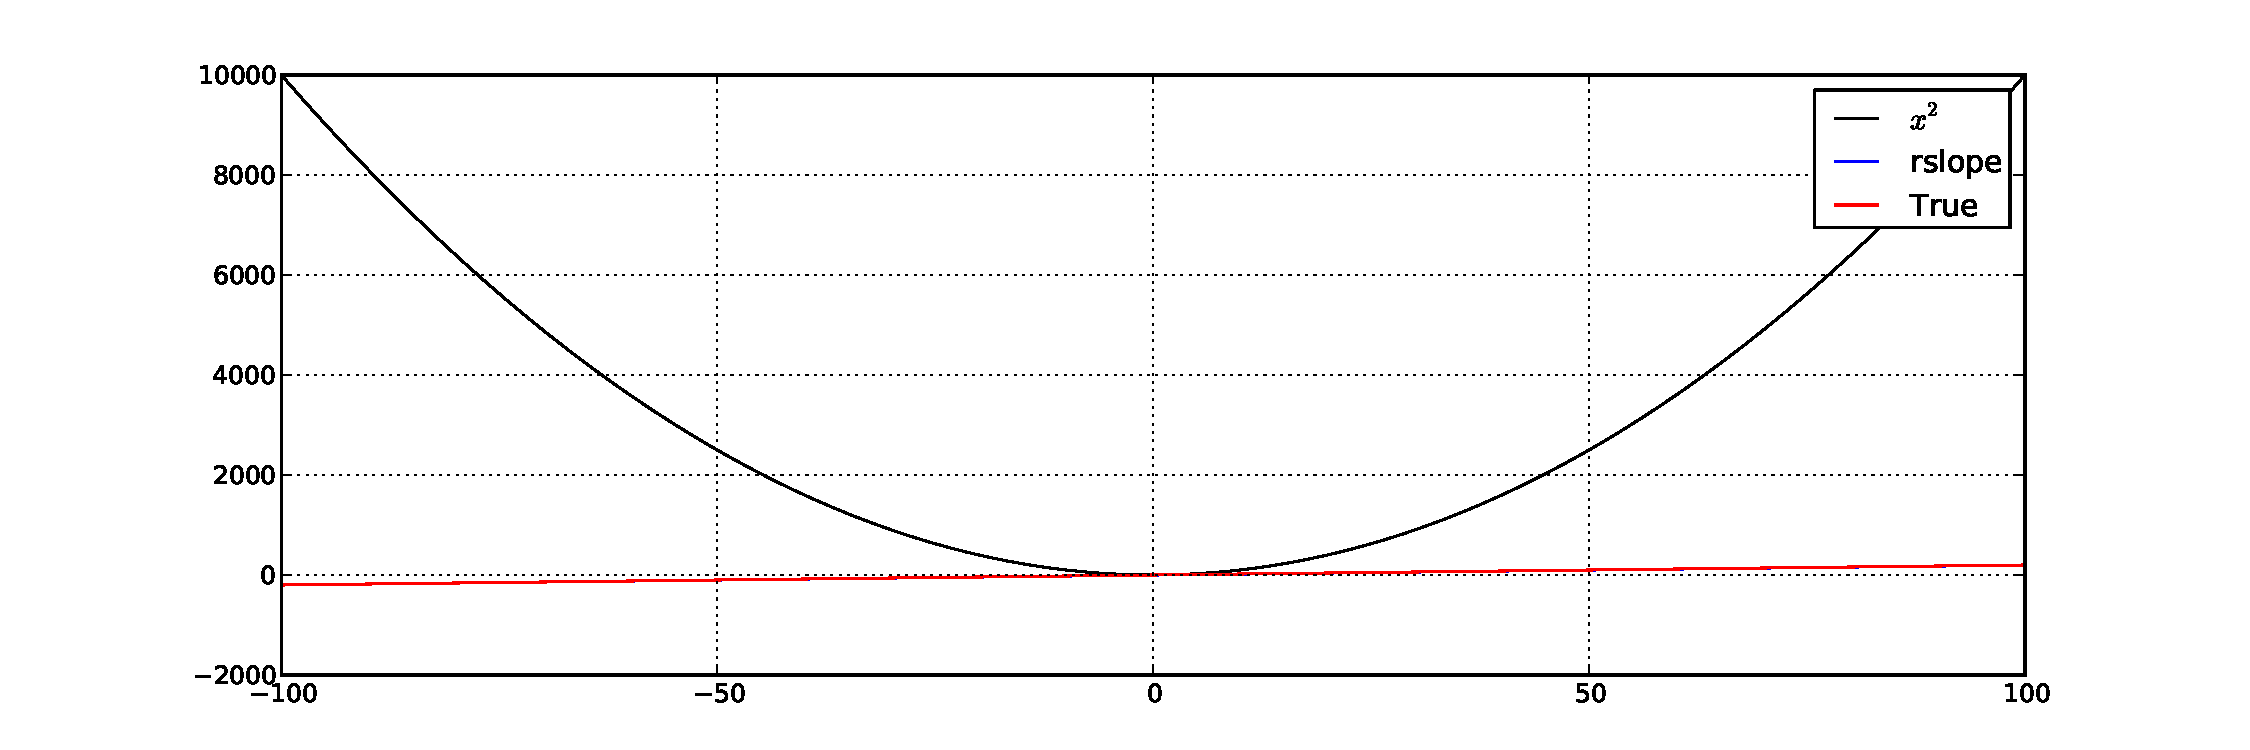
\includegraphics[scale=0.4]{xsq_test.pdf}}
\captionof{figure}{Running average slope of $f(x) = x^2$.  Output is expected with mentioned small end effects for the first and last $w$ points.}
\label{xsq_test}
\end{minipage}


\noindent%
\begin{minipage}{\linewidth}
\makebox[\linewidth]{%
      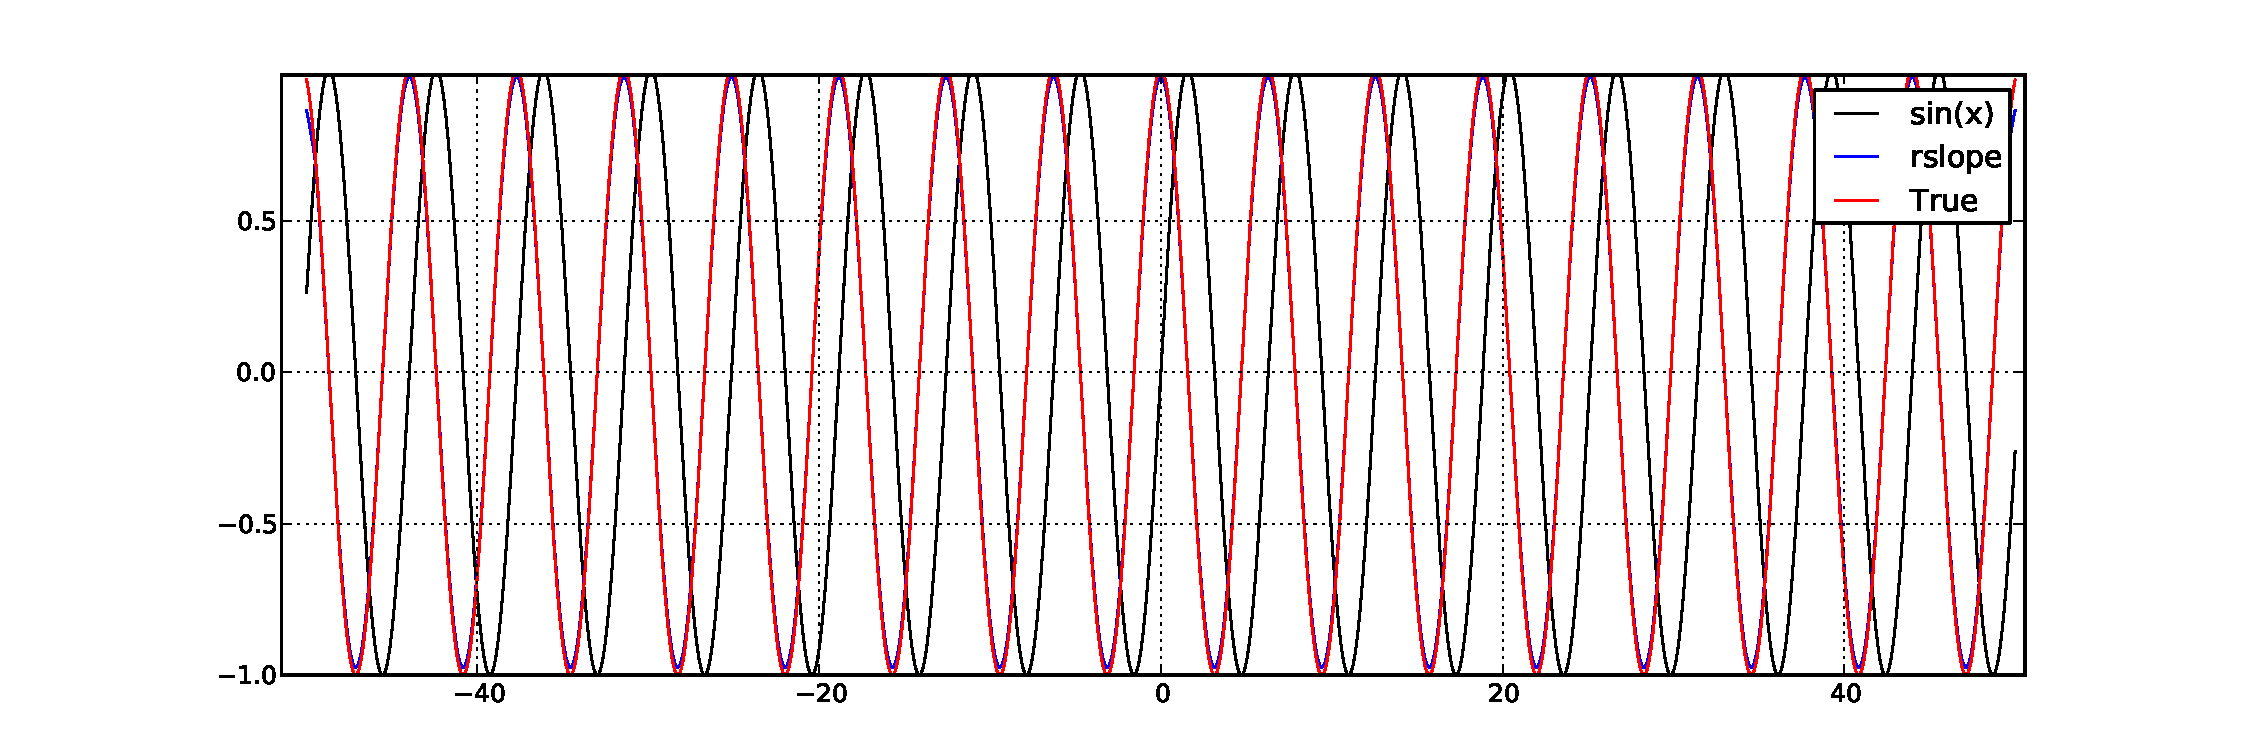
\includegraphics[scale=0.4]{sin_test.pdf}}
\captionof{figure}{Running average slope of $f(x) = \text{sin}(x)$.  Output is expected with mentioned small end effects for the first and last $w$ points.}
 \label{sin_test}
\end{minipage}



\section{Acknowledgements}
Thank you to Chris Marone (Penn State) for providing his C code for rslope and discussion of implementation.  This code is free for all to use with proper acknowledgement.  Please send any bug reports to kd5wxb@gmail.com.

\newpage

\section{Code}
\begin{lstlisting}
def rslope(x,y,window):
    """
    Takes a data vector and a window to produce a vector of the running average slope.
    The window specifies the number of points on either side of the central point, so
    the total number of points in the slope fitting is 2*window+1.  Fitting is 
    done by the least squares method where the slope is defined by the equation below.
    the beginning and ends are padded with NaN, so fewer points are in those slope 
    estimates.  Addition and subtraction to the totals is used so that the sum is not
    recomputed each time, speeding the process.
    
                    sum(x)*sum(y)
        Sum(x*y) -  -------------
                          n
    m = -------------------------
                     (sum(x))^2
        sum(x^2) - --------------
                          n
    """
    
    import numpy as np
    
    # Check that x and y are the same length
    if len(x) != len(y): 
        print "Error: x and y must be the same length"
        return 0     
    
    N = len(x) # Number of points in the dataset
    slopes = np.ones(N) # Make array for slopes
    
    # Pad data with window number of points NaN on either side
    x_padded = np.empty(2*window+N)
    x_padded[0:window] = 0
    x_padded[window:N+window] = x
    x_padded[N+window:2*window+N] = 0
    
    y_padded = np.empty(2*window+N)
    y_padded[0:window] = 0
    y_padded[window:N+window] = y
    y_padded[N+window:2*window+N] = 0
    
    sum_x    = np.sum(x_padded[0:2*window+1])
    sum_y    = np.sum(y_padded[0:2*window+1])
    sum_x_sq = np.sum(x_padded[0:2*window+1]*x_padded[0:2*window+1])
    sum_xy   = np.sum(x_padded[0:2*window+1]*y_padded[0:2*window+1])

    n = np.empty(N)
    n[0:window] = np.arange(window+1,2*window+1)
    n[window:N-window] = window*2+1
    n[N-window:N] = np.arange(2*window,window,-1)
    
    slopes[0] = (sum_xy - (sum_x*sum_y/n[0]))/(sum_x_sq - (sum_x*sum_x/n[0]))
    
    for i in range(1,N):
        sum_x    = sum_x - x_padded[i-1] + x_padded[2*window+i]
        sum_y    = sum_y - y_padded[i-1] + y_padded[2*window+i]
        sum_x_sq = sum_x_sq - x_padded[i-1]*x_padded[i-1] + \
            x_padded[2*window+i]*x_padded[2*window+i]
        sum_xy   = sum_xy - x_padded[i-1]*y_padded[i-1] +\
            x_padded[2*window+i]*y_padded[2*window+i]
        slopes[i] = (sum_xy - (sum_x*sum_y/n[i]))/(sum_x_sq - (sum_x*sum_x/n[i]))
    return slopes

if __name__ == "__main__":    
    """
    If this is called as the main program, output the derivative to the screen.
    """
    import sys
    import numpy as np
    
    if len(sys.argv) != 2:
        print "ERROR: Include a file name for the program to run on, or import"
        print "it as a module. \n"
        print "Usage:"
        print "python rslope.py filename.txt OR TO SAVE python rslope.py filename.txt > output.txt"
        print "In a script: from rslope import *"
        sys.exit(0)
    
    infile = sys.argv[1]

    try:
        x,y = np.loadtxt(infile, unpack=True)
    except:
        print "Error in file format! Two columns of numbers only! Space delimited for x y."
        sys.exit(0)
        
    window = input('Enter window length (number of points on each side of datapoint to be used): ')
    derv = rslope(x,y,window)
    
    # Output to screen
    for item in zip(x,y):
        print "%f %f"%(item[0],item[1])
\end{lstlisting}

\end{document}